\chapter{Methodology and Implementation}
\label{chap:implementation}
 
In this chapter the implementation of the GraphSLAM algorithm is presented and explained. The implementation created is capable of solving the SLAM problem in an offline manner for a 2D scenario, in the cases of known and unknown data association.

The g$^2$o framework used in this work provides of a least squares solver for the optimization of equation~\eqref{eq:minimization}, as well as a protocol to define a graph in the SLAM problem. g$^2$o is well optimized and it has several options for the solver, so the known correspondence version of the GraphSLAM algorithm is relative straightforward to implement.

However, g$^2$o doesn't provide a way to handle unknown data association, so the main goal of this work is to implement a method for solving the correspondence problem in an efficient manner.

\section{The g$^2$o Protocol}

The first step to implementing the GraphSLAM algorithm is to define a protocol to store and interpret the data on a graph. g$^2$o already provides such protocol. The stored data comes in two types: data from nodes, and data from edges. 

In SLAM context, nodes itself can be of two types, pose nodes and landmark nodes. Pose nodes represent the pose of the robot, in the 2D case they consists in 3 variables: robot's $x$ and $y$ position, and robot's bearing $\theta$. In g$^2$o a pose node is denoted with the keyword \texttt{VERTEX\_SE2}\footnote{Vertex is synonymous of node. SE2 is the Non-Euclidean space that consists of two spatial dimensions and a angular dimension.}. Landmark nodes represent the 2D position ($x$ and $y$) of a landmark. They are denoted with the keyword \texttt{VERTEX\_XY}.

Edges represents either robot's odometry (data of robot's change in position), or robot's measurements of landmarks. Odometry is measured as the difference between robot's pose at two consecutive timesteps: $(\Delta x, \Delta y, \Delta \theta)$. On the other hand, robot measurement are given as the $x$ and $y$ distance to the landmark relative to the robot reference frame. Figure~\ref{fig:protocol} illustrates the odometry an measurement of a robot. Keywords \texttt{EDGE\_SE2} and \texttt{EDGE\_SE2\_XY} are use to denote odometry and measurement edges respectively.

\begin{figure}[htbp!]
    \centering
    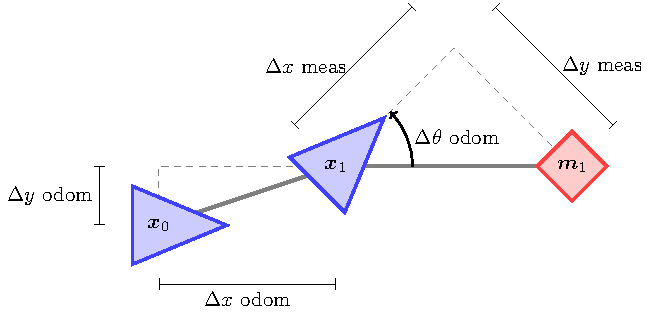
\includegraphics[width=0.7\textwidth]{tikz/protocol.pdf}
    \caption{Ilustration of odometry and measurements values in g$^2$o.}
    \label{fig:protocol}
\end{figure}

For GraphSLAM to work correctly, one must also provide to the algorithm of the uncertainty of odometry and measurements. These correspond to the covariance matrices $\bs{R}_k$ and $\bs{Q}_k$ from motion~\eqref{eq:motion-model} and measurement~\eqref{eq:measurement-model} model respectively. Actually g$^2$o works with the inverse of the covariance matrix, known as the information matrix, however, these representation are equivalent in terms of the knowledge of the system. Since covariance matrices (and their inverse) are symmetrical, only the upper diagonal elements are needed. In this work it is assumed that the model's uncertainly are time independent, i.e., all nodes have the same values for the information matrix. The notation of each element of the matrices is shown as follows:

\begin{equation}
    \bs{R}^{-1}_k = \begin{pmatrix}
    ipxx & ipxy & ipxt\\
    ipxy & ipyy & ipyt\\
    ipxt & ipyt & iptt
    \end{pmatrix} \;\;
    \bs{Q}^{-1}_k = \begin{pmatrix}
    ilxx & ilxy\\
    ilxy & ilyy
    \end{pmatrix} 
    \label{eq:info-matrices}
\end{equation}

Finally, nodes must be indexed so they can be distinguishable form other nodes, indicated by an integer \texttt{id}. Ids are used in edges to indicate the two nodes that the edge is connecting.

Table~\ref{tab:protocol} summarize the g$^2$o notation to represent nodes and edges:

\begin{table}[htbp!]
    \centering
    \begin{tabular}{|c|c|}
        \hline
        Graph element & Notation\\
        \hline
        Pose node & \texttt{VERTEX\_SE2 id x y t}\\
        Landmark node & \texttt{VERTEX\_SE2\_XY id x y}\\
        Odometry edge & \texttt{EDGE\_SE2 id1 id2 dx dy dt ipxx ipxy ipxt ipyy ipyt ipyy}\\
        Measurement edge & \texttt{EDGE\_SE2\_XY id1 id2 dx dy ilxx ilxy ilyy}\\
        \hline
    \end{tabular}
    \caption{g$^2$o protocol for node and edge definition.}
    \label{tab:protocol}
\end{table}

In a SLAM problem one usually have only information about robot odometry and measurement, so only edges data is known. All the data can be written in a plain text, that can be latter uploaded to the g$^2$o framework.

\section{The Known Correspondence Case}

Using g$^2$o solving the known correspondence case is just a matter of loading the data to the framework, set the desired parameters, and running the solver. 

The parameters that can be set in the solver includes: 

\begin{enumerate}
    \item The sparse solver for the inversion in~\eqref{eq:linear-system}: Cholesky solver, PCG solver
    \item The optimization algorithm for solving~\eqref{eq:linearized}-\eqref{eq:update}: Gauss-Newton, Levenberg-Marquardt
    \item The number of iteration for the algorithm to stop.
\end{enumerate}

For the sparse solver, g$^2$o uses third-parties libraries from which the user can choose: CHOLMOD, CSparse\footnote{CHOLMOD and CSparse can be found in \url{http://faculty.cse.tamu.edu/davis/suitesparse.html}}, Eigen\footnote{\url{http://eigen.tuxfamily.org/index.php?title=Main_Page}}. 

This work provides of a Python script to easily set the parameters of the framework and run the solver. It also provides of a 2D simulator that generates a robot path, landmarks and measurements. It's a modified version of the g$^2$o simulator that allows the user to set the information parameters from matrices~\eqref{eq:info-matrices} in the simulations. This make possible to test the GraphSLAM algorithm for different noise levels. The simulation also allows to compare the results with the ground truth (the true values of the robot path and landmarks generated by the simulator). 

The Python script is also able to generate an initial guess of the estimate using robot odometry and the first measurement of each landmark. The initial guess is necessary for the optimization algorithm to work. Figure~\ref{fig:simulation} shows an example of the ground truth and the initial guess of a SLAM simulation.

\begin{figure}[htbp!]
    \centering
    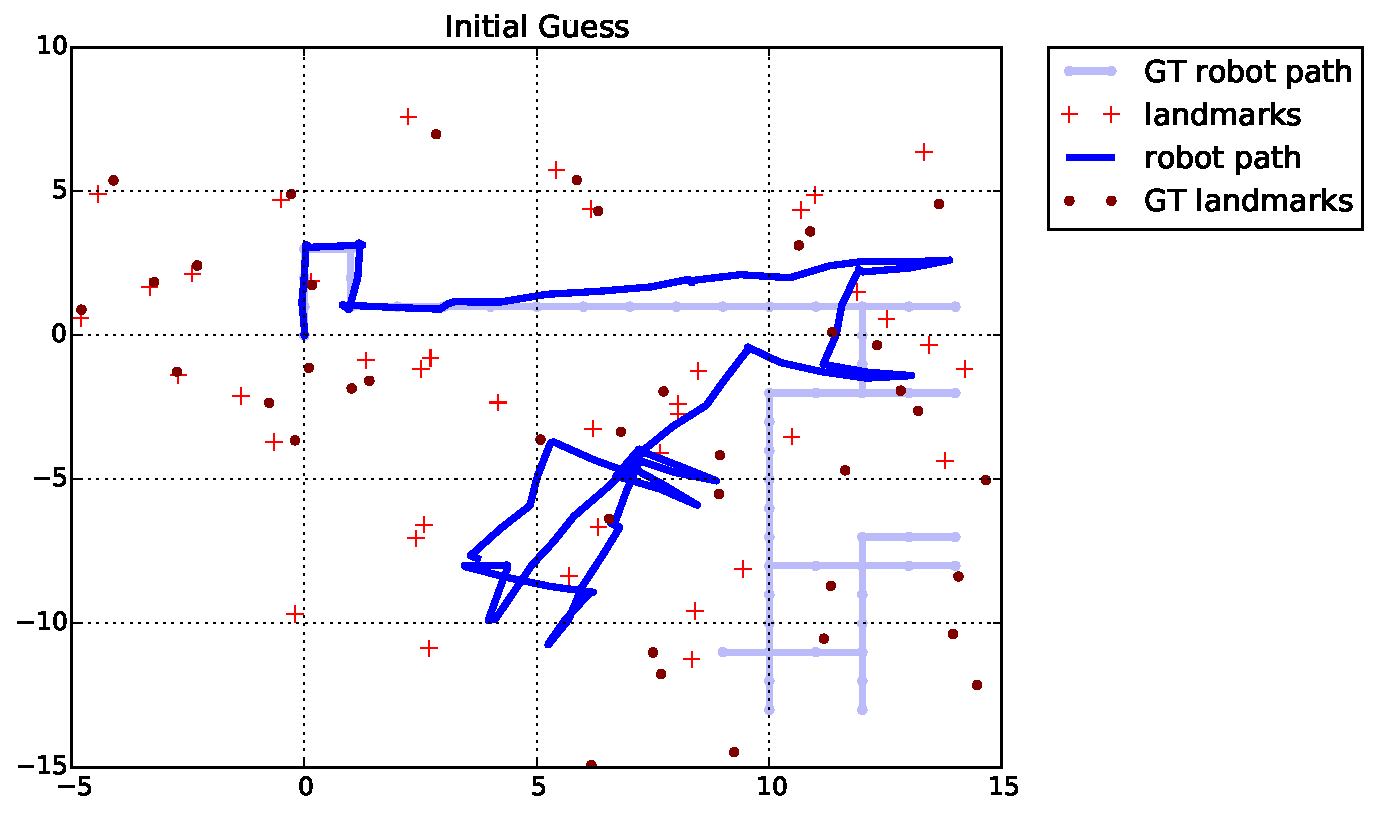
\includegraphics[width=0.8\textwidth]{imagenes/guess_op_100_oa_100_lp_100_ds_100.pdf}
    \caption{Example of an SLAM simulation. The light blue line is ground truth path, and dark red circles are ground truth landmark. The blue line is odometry path, red cross are initial guess landmarks.}
    \label{fig:simulation}
\end{figure}

The pseudocode for the known correspondence case is shown in Algorithm~\ref{alg:known-correspondence}.

\begin{algorithm}
    \caption{GraphSLAM Known Correspondence}
    \label{alg:known-correspondence}
    \begin{algorithmic}[1]
        \Require optimizer, data
        \State optimizer.setParameters(parameters)
        \State optimizer.loadData(data)
        \State optimizer.genInitialGuess()
        \State optimizer.solve(numberIterations)
        \State optimizer.writeData()
    \end{algorithmic}
\end{algorithm}

Optionally g$^2$o can use robust kernels to deal with outliers. An outlier is a corrupt measurement that doesn't follows the distribution assumed for the model. They are usually generated by sensors malfunctions and tend to have extreme values, far away form the expected measurement. 

From equation~\eqref{eq:simplified}, it can be seen that each error function has a quadratic influence in function $F(\bs{y})$. This means that a single outlier can significantly degrade the construction of $F$, and thus the result of the estimation. To mitigate this problem a robust kernel function can be applied to each error term $\bs{e}_{ij}(\bs{y})$ in~\eqref{eq:simplified}, so that high values of $\bs{e}_{ij}$ has reduced effect in $F$. Robust kernels included in g$^2$o are: Cauchy, DCS, Fair, GemanMcClure, Huber, PseudoHuber, Saturated, Tukey, Welsch. Most robust kernels must also specify the kernel's width, that is the point on the function in which the kernel effect start. Figure~\ref{fig:kernels} shows the plots of different kernels in g$^2$o. 

\begin{figure}[htbp!]
    \centering
    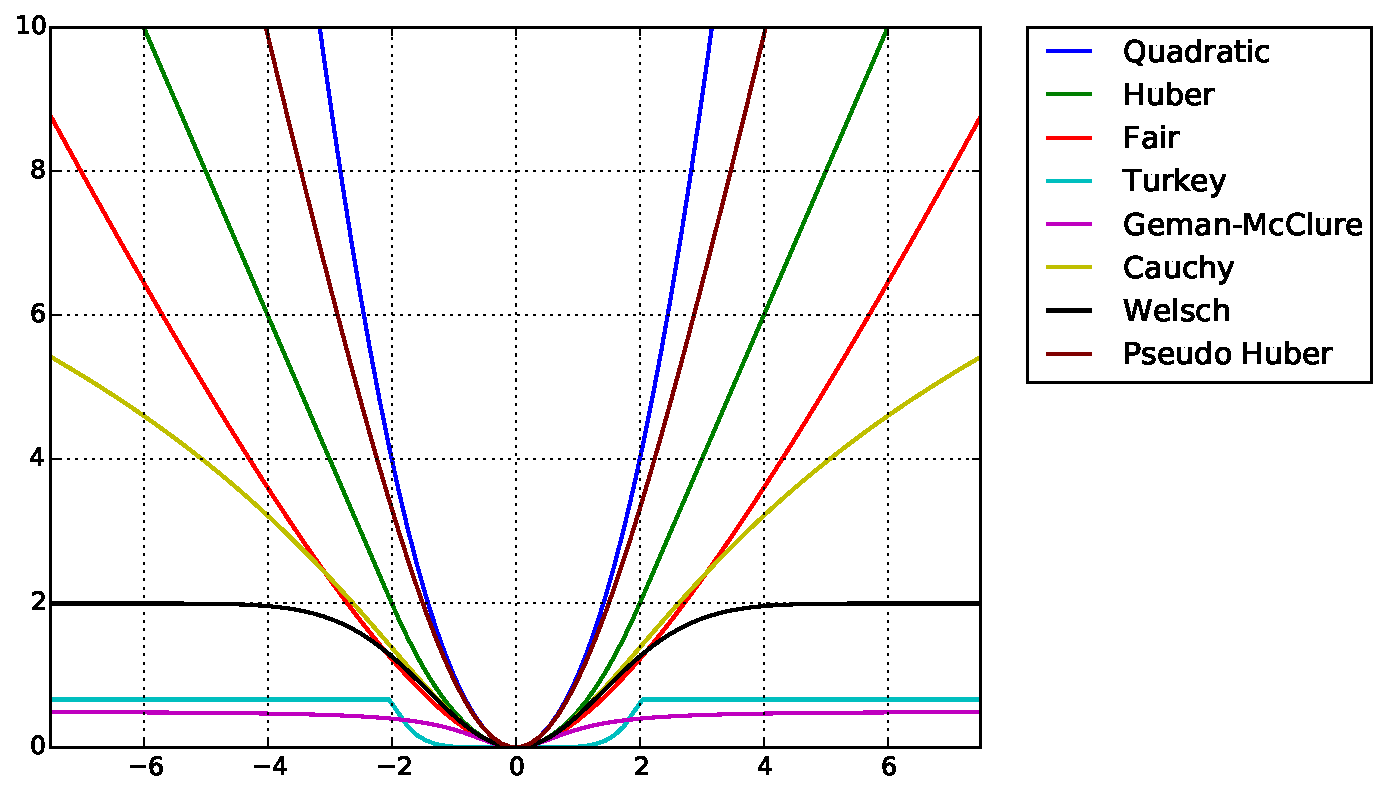
\includegraphics[width=0.8\textwidth]{imagenes/kernels.pdf}
    \caption{Plots of different robust kernels with equals width, compared with the quadratic function.}
    \label{fig:kernels}
\end{figure} 

In this work a Huber kernel of width 1 is used.

\section{The Unknown Correspondence Case}

In the unknown correspondence case there is no information of which landmark generates each measurement, neither of how many landmarks are in the map. The g$^2$o framework does not provides a way to solve the correspondence problem, so a method must be developed to address de issue. In this work the method implemented is based in the one presented in~\cite{graphslam}, with some differences to take in account the speed,  false alarms\todo{review}. 

\subsection{The Correspondence Test}

The premise of the method is as follows: a correspondence test is developed to check the likelihood of two landmarks being the same. If the likelihood is high enough, the landmarks are merged into one. 

To justify mathematically the correspondence test the variable $\bs{\Delta}_{j,k}=\bs{m}_j-\bs{m}_k$ is defined as the difference in position of landmark $\bs{m}_j$ and $\bs{m}_k$. The posterior probability of $\bs{\Delta}_{j,k}$ over the measurements and control inputs is given by:

\begin{equation}
p(\bs{\Delta}_{j,k}|\bs{z}_{1:k},\bs{u}_{1:k})=
\det(2\pi \bs{\Sigma}_{\bs{\Delta}_{j,k}})^{-\frac{1}{2}}\exp\left\lbrace -\frac{1}{2}(\bs{\Delta}_{j,k}-\bs{\mu}_{\bs{\Delta}_{j,k}})^T
\bs{\Sigma}_{\bs{\Delta}_{j,k}}^{-1}(\bs{\Delta}_{j,k}-\bs{\mu}_{\bs{\Delta}_{j,k}})\right\rbrace
\label{eq:correspondence-test}
\end{equation}

Where $\bs{\mu}_{\bs{\Delta}_{j,k}}$ is the current estimate of the landmark's difference. It can be easily computed as $\bs{\mu}_{\bs{m}_j}-\bs{\mu}_{\bs{m}_k}$, where $\bs{\mu}_{\bs{m}_j}$ and $\bs{\mu}_{\bs{m}_k}$ are the current estimate of both landmarks.

Matrix $\bs{\Sigma}_{\bs{\Delta}_{j,k}}$ is the covariance matrix marginalized over landmarks $j$ and $k$. Since it has been assumed a normal distribution for the estimate, $\bs{\Sigma}_{\bs{\Delta}_{j,k}}$ can be computed using the marginalization lemma~\cite{graphslam}. In practice, g$^2$o provides a function to compute $\bs{\Sigma}_{\bs{\Delta}_{j,k}}$.

\todo[inline]{explain marginal cov equation?}

When two landmarks are equivalent it is expected that their position is the same, hence $\Delta_{j,k}=0$. Evaluating this in the posterior probability~\eqref{eq:correspondence-test} gives the likelihood of landmark equivalence:

\begin{equation}
\pi_{j=k} \defi
p(\bs{\Delta}_{j,k}=0|\bs{z}_{1:k},\bs{u}_{1:k})=
\det(2\pi\bs{\Sigma}_{\bs{\Delta}_{j,k}})^{-\frac{1}{2}}
\exp\left\lbrace-\frac{1}{2}\bs{\mu}_{\bs{\Delta}_{j,k}}^T\bs{\Sigma}_{\bs{\Delta}_{j,k}}^{-1}\bs{\mu}_{\bs{\Delta}_{j,k}}\right\rbrace
\end{equation}

Then the correspondence test consist in assert a landmark equivalence when the likelihood $\pi_{j=k}$ is grater that a user defined threshold $\chi$. Intuitively a greater threshold means being more strict in considering a landmark merging.

\subsection{The Unknown Correspondence Algorithm}

Once the correspondence test is defined, it can be used to implement an GraphSLAM algorithm with unknown data association. 

The algorithm works as follows: first all landmarks are initialized as if each measurement correspond to an individual landmark. The correspondence test is run over every possible pair of landmarks, merging landmarks who pass the test. After the tests are finished, the estimate is updated running the solver in the same way as in the case of known correspondence. Then the correspondence test is run again and the solver is run afterward. Correspondence test and solver are alternated until no more landmark associations are found. 

Algorithm~\ref{alg:unknown-correspondence} presents the unknown correspondence algorithm in pseudocode. 

\begin{algorithm}
    \caption{GraphSLAM Unknown Correspondence}
    \label{alg:unknown-correspondence}
    \begin{algorithmic}[1]
        \Require optimizer, data
        \State optimizer.setParameters(parameters)
        \State optimizer.loadData(data)
        \State optimizer.genInitialGuess()
        \State
        \While{association found} 
            \ForAll{pair of landmark ($j$,$k$)} 
                \If{correspondenceTest($j$,$k$) $\geq \chi$} 
                    \State optimizer.merge($j$,$k$) 
                \EndIf 
            \EndFor
            \State optimizer.solve(numberIterations)
        \EndWhile
        \State
        \State optimizer.writeData()
    \end{algorithmic}
\end{algorithm}

\subsection{Speeding up the Unknown Correspondence Algorithm}

Algorithm~\ref{alg:unknown-correspondence} is inefficient. In particular the correspondence test is run over every pair of landmarks at each iteration. The possible pairs is quadratic in the number of landmarks, furthermore, even landmarks that are obviously not equivalent, such as landmarks greatly separated, are tested. Empirical testing have shown that the bottleneck of the algorithm is the the correspondence test, in particular, the computation of the marginalized covariance $\bs{\Sigma}_{\bs{\Delta}_{j,k}}$, so is necessary call this function as less as possible. The optimization of the algorithm is essential to run GraphSLAM in large datasets. The next subsections presents the strategies adopted to improve the algorithm performance.

\subsubsection{Incremental Optimization}

\subsubsection{Distant Test}

\subsubsection{Late Landmark Merging}